\newcommand{\CLASSINPUTbaselinestretch}{1.5}
\newcommand{\CLASSINPUTinnersidemargin}{25mm}
\documentclass[12pt, conference]{IEEEtran}
\usepackage{algorithmic}
\usepackage{amsfonts}
\usepackage{amsmath}
\usepackage{amssymb}
\usepackage{caption}
\usepackage{graphicx}
\usepackage{hyperref}
\usepackage{listings}
\usepackage[lighttt]{lmodern}
\usepackage{subcaption}
\usepackage{textcomp}
\usepackage{xcolor}

\lstset{basicstyle=\ttfamily, keywordstyle=\bfseries}

\begin{document}

\begin{abstract}
\end{abstract}

\section{Introduction}
The scanning electron microscope (SEM) is a type of microscope that produces images using signals generated from the interaction between electrons and the surface under observation. Higher resolution can be achieved compared to the traditional optical microscope since electrons have much lower wavelength than light. An SEM can have a resolution lower than one nanometre, whereas that of an optical microscope is often limited to a few hundred nanometres. This has benefited a variety of fields. For example, scientists have been using the SEM to analyse the doping density in semiconductors \cite{SEM for semiconductors} and to view changes in bacterial cells \cite{SEM for bacterial cells}.

Fig. \ref{SEM basic construction} shows the basic construction of an SEM. The electron gun generates an electron beam, which is transformed into an electron probe after passing through the condenser lens and objective lens. It is scanned across the specimen under the effect of the scanning coil. As a result of the interaction between the incident electrons and the specimen, some electrons are emitted from the specimen. These are called secondary electrons and are collected by the detector, which generates signals whose magnitudes depend on the strength of the secondary electrons. The display unit produces one image after each complete scan of the specimen.

\begin{figure}[htbp]
    \centering
    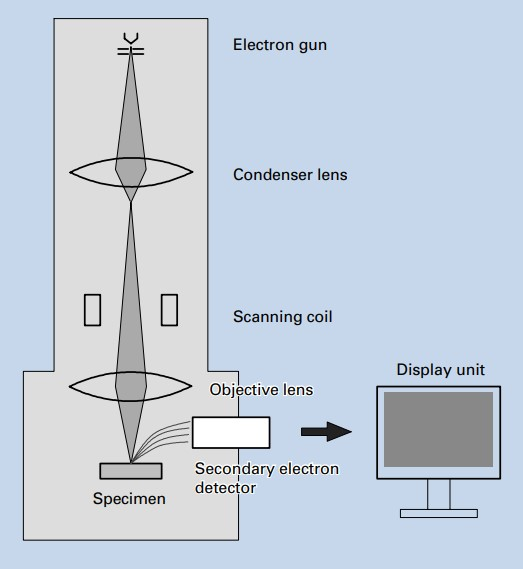
\includegraphics[width=0.45\textwidth]{Images/SEM basic construction.jpg}
    \caption{Basic construction of an SEM \cite{SEM A to Z}.}
    \label{SEM basic construction}
\end{figure}

Digital image analysis methods have been widely used in the field of SEM. For example, the fibre orientation distribution of non-woven fabrics can be determined using fast Fourier transform (FFT) and Hough transform (HT) \cite{SEM for microstructural analysis}. The FFT is an especially popular algorithm and many papers have been published on the use of it. However, due to its complexity and a lack of fast hardware, real-time analysis had largely been impossible or impractical in the past, i.e. it was only feasible to perform FFT on images off-line. In 1997, with an advanced central processing unit (CPU) --- the Pentium Pro, it was only possible to achieve a refresh rate of about 0.6 frames per second for an 8-bit 1024 $\times$ 1024 image \cite{SEM image sharpness measurement}. The enhancement of CPUs has enabled faster frame rates and more recently, the development of the graphics processing unit (GPU) has taken image analysis to a different level.

The GPU was originally designed to efficiently manipulate data in order to accelerate the rendering of 3D images on displays. Depending on the position, pixels in a 3D image may require different processing to achieve effects such as lighting, blurring, and fogging. This is achieved by breaking down the image into a massive number of fragments and processing each fragment individually. The processes happen independently but may share the same logical sequence of control, and this pattern is named single instruction multiple data (SIMD). A GPU consists of a large array of processing cores, with each of them using SIMD to process a block of fragments.

The characteristic of the GPU allows it to outperform central processing units (CPUs) when performing algorithms that manipulate data in parallel. Take the dot product between two vectors of size 1000 as an example, the processing cores on the GPU might be 100 times slower than the CPU, but if 1000 of them work in parallel and each computes the multiplication of one element from each vector, the overall speed will be 10 times faster. This has allowed computer vision programs that were previously impossible or computationally too expensive to build. For example, a wearable mediated reality device that makes computer-generated information appear to the user as though it was anchored in the real world \cite{GPU mediated reality}.

The goal of the project is to develop software tools based on fast computation provided by the GPU, to support interactive real-time diagnosis of SEM images that assists the operator or automated procedures, with a focus on the use of FFT.

\section{Software aspects of the tools}
\subsection{Design principle}
Considering that the work of the project may serve as the foundation stone for many further developments, the design of the software has a strong emphasis on readability and maintainability.

\subsection{The selection of programming language}
The SEM used for the project is made by Carl Zeiss AG, which provides an application programming interface (API) that can be used for controlling the SEM and grabbing images from it. The API supports C++ and thus makes it a possible programming language for the project. Being a relatively low-level compiled language makes C++ extremely fast and useful for speed-critical applications. However, it also means that C++ has a complex syntax, which could significantly slow down development if the user does not have enough experience with it.

Considering the time scale of the project and to make development easier for people who will continue the work, Python is selected instead as the programming language, which has a much simpler syntax and is widely supported. With careful design, it has proved to be able to produce useful results despite the slower speed (see later sections).

\subsection{Modules of the software}
The software is highly modularised, which maximises readability and maintainability. This also makes it easier to translate the programs into C++ later if better performance is needed since C++ is mostly used in an object-oriented manner. Fig. \ref{Software class diagram} shows the six main classes of the software.

\begin{figure}[htbp]
    \centering
    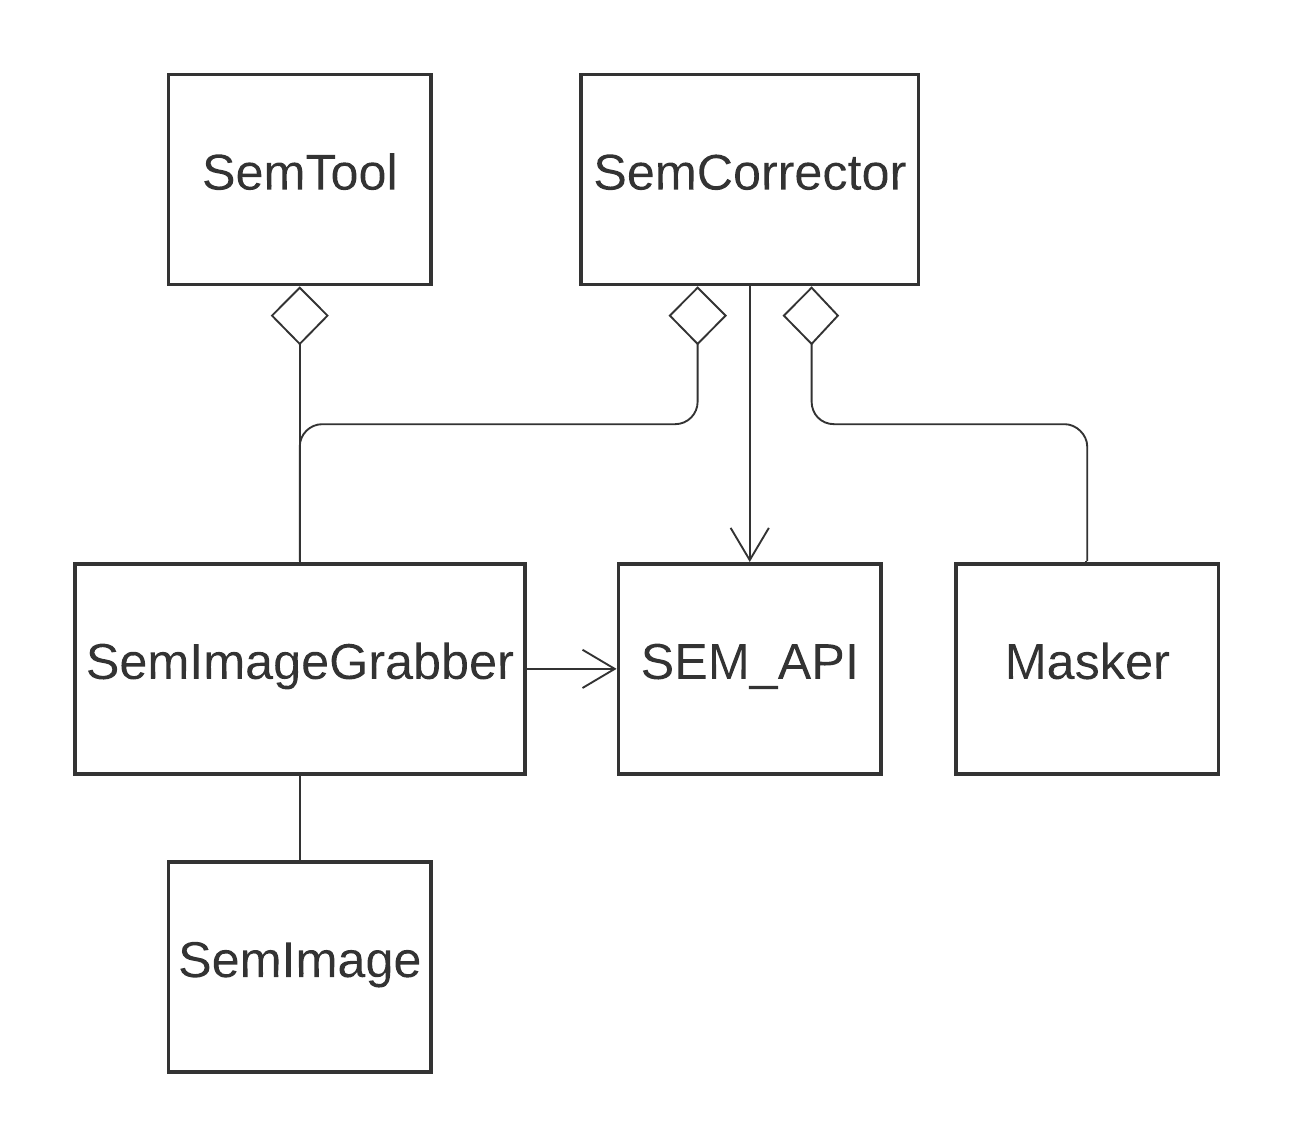
\includegraphics[width=0.45\textwidth]{Images/Software class diagram.png}
    \caption{Class diagram of the software in unified modelling language (UML).}
    \label{Software class diagram}
\end{figure}

\textit{SEM\_API} is a Python wrapper for the native SEM API written by Luyang Han, which allows the user to directly control the SEM in Python.

\textit{SemImage} encapsulates variables and methods that are directly relevant to an image taken by the SEM, and \textit{SemImageGrabber} is a helper class that helps obtain image data from the SEM and create instances of \textit{SemImage} from them. Images can be obtained in two ways:
\begin{itemize}
    \item From the SEM.
    \item From a local folder, which is helpful when the SEM is not available.
\end{itemize}
\textit{SemImageGrabber} detects if the SEM is available and decides on which way to use.

\textit{SemTool} handles the creation and rendering of the graphical user interface (GUI). Fig. \ref{Software GUI} shows a screenshot of the control panel. The pushbuttons open a window for the corresponding plot and the radio buttons select algorithms (see section \ref{Section histogram equalisation} and \ref{Section FFT} for detailed descriptions) to be performed on the image. The plots are shown on different windows and can be opened and closed individually. This improves framerate by allowing the user to close unneeded windows, and also makes it easier to add other plots later. Table \ref{Software framerates} shows that the improvement is rather significant, as rendering windows is a major time-consuming process of the software. When only one window is opened, a refresh rate of about 16 frames per second is possible.

\begin{figure}[htbp]
    \centering
    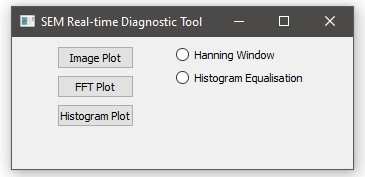
\includegraphics[width=0.45\textwidth]{Images/Software screenshot.jpg}
    \caption{Screenshot of the GUI.}
    \label{Software GUI}
\end{figure}

\begin{table}[htbp]
    \caption{Results of software framerate test}
    \begin{center}
    \begin{tabular}{|c|c|}
    \hline
    \textbf{Number of} & \textbf{Time taken to} \\
    \textbf{plots opened} & \textbf{update each frame} \\
    \hline
    zero & 15 ms \\
    \hline
    one & 60 ms \\
    \hline
    three & 160 ms \\
    \hline
    \multicolumn{2}{l}{$^{\mathrm{a}}$The numbers are approximate.} \\
    \multicolumn{2}{l}{$^{\mathrm{b}}$With 8-bit grey-scale 1024 $\times$ 768 input images.} \\
    \multicolumn{2}{l}{$^{\mathrm{c}}$With Intel Core i7 and NVIDIA GTX 1060.}
    \end{tabular}
    \label{Software framerates}
    \end{center}
\end{table}

There are two ways for updating the plots, and the first one is to re-render the whole window. This wastes time since some components are always the same and do not need to be re-rendered, such as the window title and the axes. Therefore, \textit{SemTool} uses the second method, where only the data to be plotted are updated. This directly modifies the relevant data in the memory of the GPU, thereby avoiding re-rendering the whole window. Tests have shown that if the first method is used, the time taken to update each frame when there is only one plot opened will be 90 ms instead of 60 ms.

\textit{SemCorrector} implements the automatic focusing and astigmatism correction algorithm and uses a helper class \textit{Masker} to achieve fast computation (see section \ref{Section correction algorithm} for detailed descriptions). Due to the impact of the COVID-19 pandemic, the algorithm has not been fully tested and is therefore not integrated to the GUI yet.

\subsection{Method to utilise the GPU}
As the popularity of using GPU to perform general-purpose processing increases (GPGPU), GPU manufacturers have started providing APIs that make writing GPU code easier. The project uses the CUDA Toolkit made by NVIDIA and the Python library \textit{CuPy}. \textit{CuPy} is an implementation of multi-dimensional arrays on CUDA, and one of its main advantages is that its core multi-dimensional array class is largely compatible with the Python \textit{NumPy} library. This allows existing code to be easily converted to harness the power of the GPU.

\section{Real-time histogram equalisation for improving image contrast}
\label{Section histogram equalisation}
There are many types of histograms in image processing. The grey level (brightness level) pixel intensity histogram, which plots the number of pixels of each grey value in the image, is the most relevant one for SEM images. This is because an SEM translates the energy of the secondary electrons directly into a grey level, colours do not exist in SEM images.

The algorithm for obtaining the histogram of an SEM image is given by
\begin{equation}
    n_l = \frac{1}{P} \sum_{p} I(l_p=l),
\end{equation}
where $n_l$ is the normalised number of pixels of grey level $l$, $P$ is the total number of pixels in the image and $l_p$ is the grey level of the $p_{th}$ pixel. 

Fig. \ref{C original} shows an 8-bit grey-scale image, i.e. its depth of digitisation is 8-bit and it has 256 grey levels. Fig. \ref{C original histogram} shows the histogram of the image and its integral. As can be seen in the histogram, most pixels are concentrated in the middle of the greyscale. This is reflected by the fact that the image is missing its highlights and shadows.

\begin{figure}[htbp]
    \centering
    \begin{subfigure}{0.4\textwidth}
        \centering
        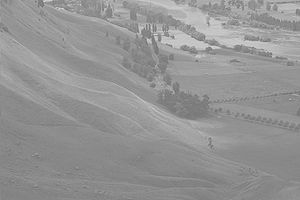
\includegraphics[width=1\textwidth]{Images/C original.jpg}
        \caption{Original image.}
        \label{C original}
    \end{subfigure}
    \begin{subfigure}{0.4\textwidth}
        \centering
        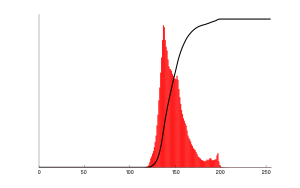
\includegraphics[width=1\textwidth]{Images/C original histogram.png}
        \caption{Histogram of the original image.}
        \label{C original histogram}
    \end{subfigure}
    \begin{subfigure}{0.4\textwidth}
        \centering
        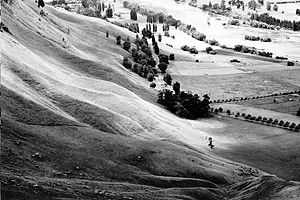
\includegraphics[width=1\textwidth]{Images/C equalised.jpg}
        \caption{Histogram-equalised image.}
        \label{C equalised}
    \end{subfigure}
    \begin{subfigure}{0.4\textwidth}
        \centering
        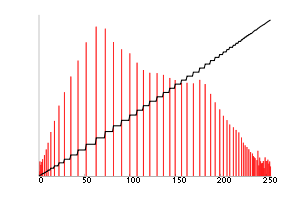
\includegraphics[width=1\textwidth]{Images/C equalised histogram.png}
        \caption{Histogram of the histogram-equalised image.}
        \label{C equalised histogram}
    \end{subfigure}
    \caption{Histogram and histogram equalisation.}
    \label{Histogram and histogram equalisation}
\end{figure}

Histogram equalisation is a method for adjusting the distribution of pixel intensities of an image, to improve its overall contrast. Effectively, it is achieved by spreading out more frequent intensity values. To perform histogram equalisation, firstly obtain the integral of the histogram using
\[s_l = \sum_{i=1}^{l} n_i,\]
where $s_l$ is the value of the integral at grey level $l$. The integral spans from 0 to 1 as the histogram is normalised. Scale the integral by the maximum grey level and perform rounding to create the transform function
\begin{equation}
    f_l = \lfloor s_lL \rfloor,
    \label{Histogram equalisation transform function}
\end{equation}
If a pixel in the original image has a grey level $l$, it will have a grey level $f_l$ in the transformed image. For example, if all pixels in the original image are concentrated between grey level 100 to 200, the pixels of level 100 will become 0 in the new image while the pixels of level 200 will become 255 (assuming an 8-bit image).

The result is more noticeable when the image has low contrast, such as the one shown in Fig. \ref{C original}. The histogram-equalised version of it is given in Fig. \ref{C equalised} and the new histogram in Fig. \ref{C equalised histogram}. More details are now visible as the contrast has been enhanced.

The most time-consuming part of histogram equalisation is to map all pixels in the original image to their new values using the transform function \eqref{Histogram equalisation transform function}. This can be implemented using CPU code in one line:
\begin{lstlisting}
newImage = 
  map(lambda x: f[x], image)
\end{lstlisting}
\lstinline{f} is an array that serves as the transformation function, if the original pixel value is x, the new value should be \lstinline{f[x]}. The \lstinline{lambda} operator is a way to create small anonymous functions, which are throw-away and are only needed where they are created. It improves conciseness and readability by reducing code bloat. \lstinline{lambda x: f[x]} creates an anonymous function that returns \lstinline{f[x]} when given \lstinline{x}, and \lstinline{map()} uses this function to transform all pixels in \lstinline{image}. This gives a time complexity of $O(N^2)$ which is not optimal. A smaller time complexity can be achieved using the GPU code:
\begin{lstlisting}
map = cupy.ElementwiseKernel(
  'T x, raw T f', 'T xNew',
  'xNew = f[x]',
  'map'
)
newImage = map(image, f)
\end{lstlisting}
\lstinline{cupy.ElementwiseKernel()} defines a kernel that the GPU uses to process the input data in parallel. Tests have shown that the use of GPU can increase the speed by 2 times, as summarised in Table \ref{Software speed comparison}. In theory, the factor of speed improvement should be similar as that for calculating the histogram, since it also requires iterating through all pixels in the image. However, the code implementations introduce overheads which limit the improvement in speed.

\begin{table}[htbp]
    \caption{Speed comparison between CPU and GPU}
    \begin{center}
    \begin{tabular}{|c|c|c|}
    \hline
    \textbf{Algorithm} & \textbf{Time taken} & \textbf{Time taken} \\
    & \textbf{using CPU} & \textbf{using GPU} \\
    \hline
    Apply Hanning window & 16 ms & 9 ms \\
    \hline
    Calculating histogram & 30 ms & 2 ms \\
    \hline
    Histogram equalisation & 9 ms & 5 ms \\
    \hline
    Fast Fourier transform & 60 ms & 8 ms \\
    \hline
    \multicolumn{3}{l}{$^{\mathrm{b}}$For an 8-bit grey-scale 1024 $\times$ 768 input image.} \\
    \multicolumn{3}{l}{$^{\mathrm{c}}$With Intel Core i7 and NVIDIA GeForce GTX 1060.}
    \end{tabular}
    \label{Software speed comparison}
    \end{center}
\end{table}

\section{Real-time fast Fourier transform for evaluating image focusing and astigmatism}
\label{Section FFT}
The quality of an SEM image is affected by aberrations. While some exist because of the fundamental properties of the microscope and are difficult to get rid of, some can be eliminated by adjusting relevant settings. Two important ones are focus and stigmator control, which directly affect the resolution and astigmatism of the image, respectively. Fig. \ref{SEM sample images} illustrates the effect of wrong focus and stigmator settings.

\begin{figure}[htbp]
    \centering
    \begin{subfigure}{0.45\textwidth}
        \centering
        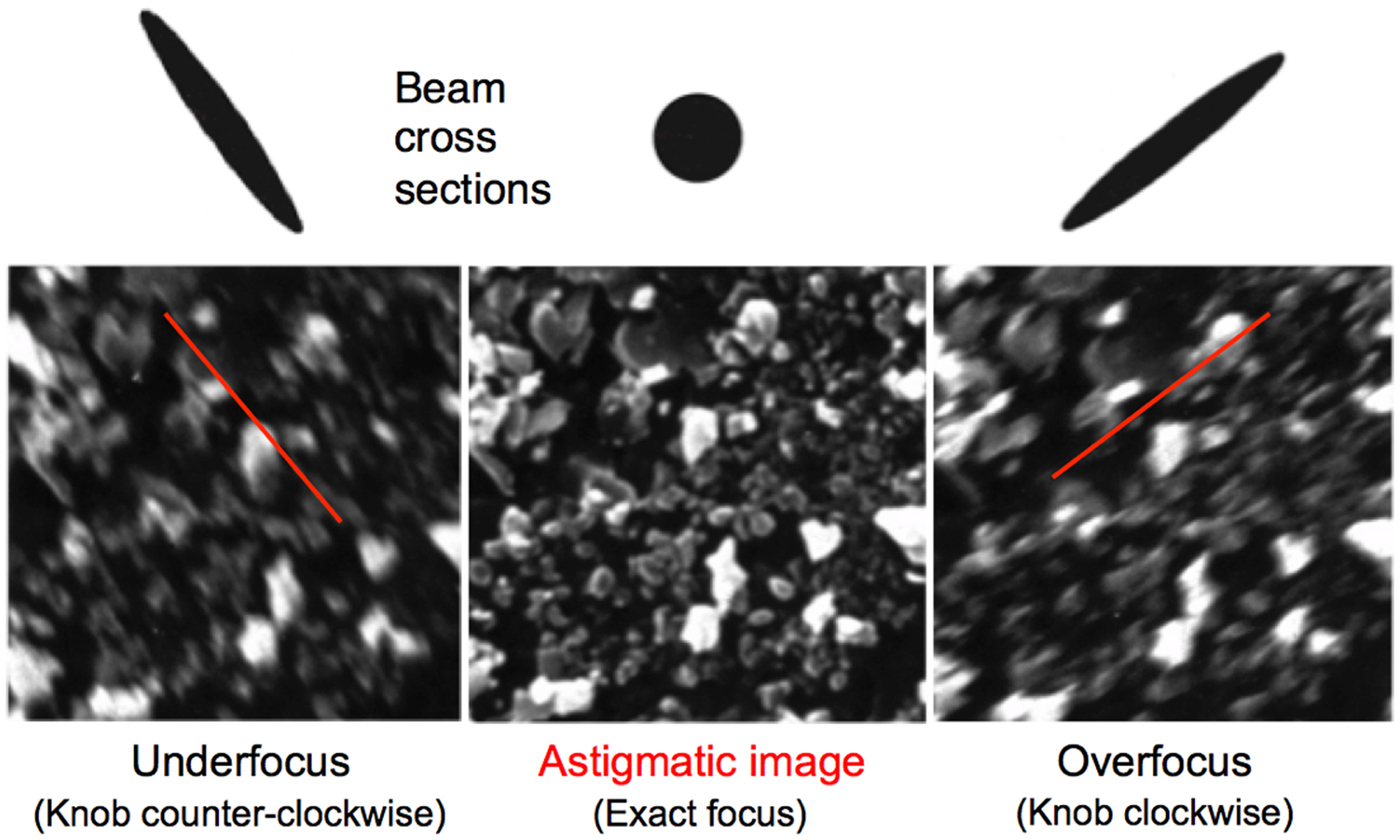
\includegraphics[width=1\textwidth]{Images/B astigmatic a.jpeg}
    \end{subfigure}
    \begin{subfigure}{0.45\textwidth}
        \centering
        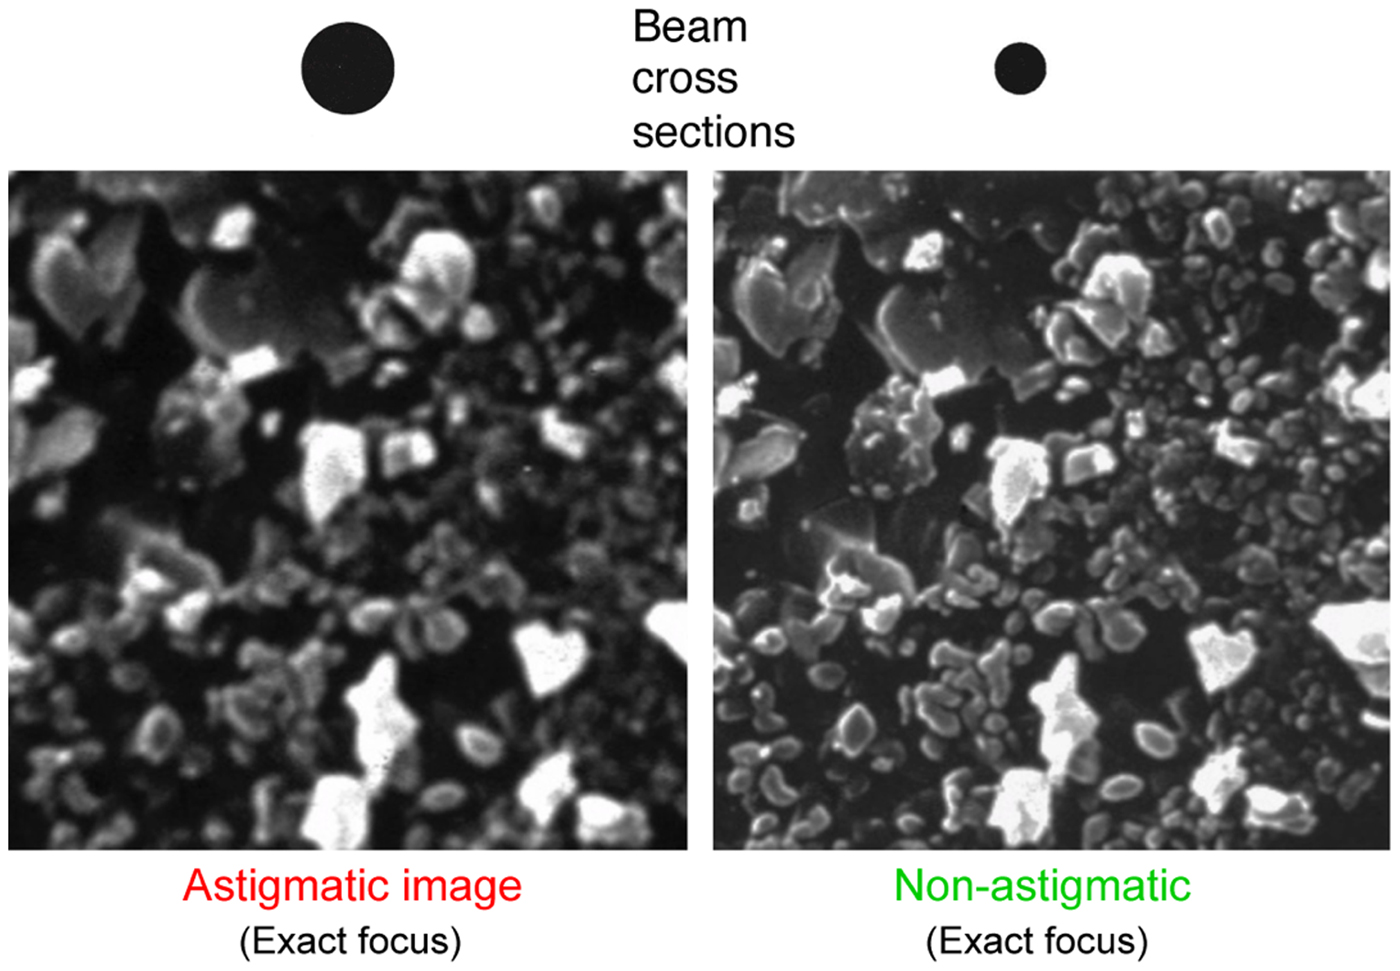
\includegraphics[width=1\textwidth]{Images/B astigmatic b.jpeg}
    \end{subfigure}
    \caption{Sample astigmatic SEM images \cite{SEM astigmatism correction}.}
    \label{SEM sample images}
\end{figure}

Focus determines the focal point of the electron probe. When the focal point is far from the surface of the specimen, the incident electrons interact with the specimen in a larger area. As a result, spots near each other produce signals of closer magnitude. This makes the image appear blurry.

Stigmators are used to compensate for astigmatism. Astigmatism arises due to imperfections in components of the SEM, and describes uneven focus in the electron probe, as shown in Fig. \ref{SEM uneven focus}. When the electron probe is out of focus, astigmatism makes the incident electrons interact with the specimen in an elliptical area, and thus makes the image appear stretched. When the electron probe is in focus, astigmatism makes the image appear blurry.

\begin{figure}[htbp]
    \centering
    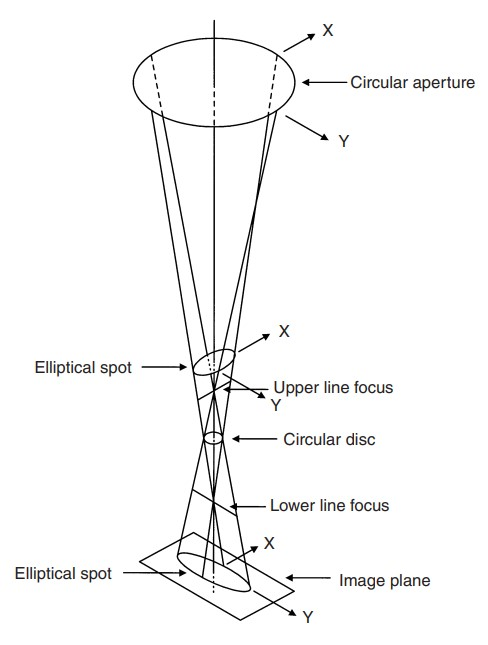
\includegraphics[width=0.45\textwidth]{Images/SEM uneven focus.jpg}
    \caption{Uneven focus of the SEM.}
    \label{SEM uneven focus}
\end{figure}

Although experienced SEM operators can often find the right settings for focus and stigmator control in a short time, it may not be as straightforward for new users. The complexity arises because any judgement of an image is based on what the operators see through their eyes, which is rather subjective. Sometimes, the surface being observed may have a complex structure and makes adjusting even harder. Intensive training and practical experience are often required for an operator to become efficient in using the SEM.

The Fourier transform (FT) decomposes a function into its constituent frequencies, as illustrated in Fig. \ref{FT}. The function in red is can be represented by a superposition of all the sinusoidal functions shown, each having a unique frequency and with magnitudes as indicated on the right panel. A function that changes more abruptly will have stronger high-frequency components than a smoother one. 

\begin{figure}[htbp]
    \centering
    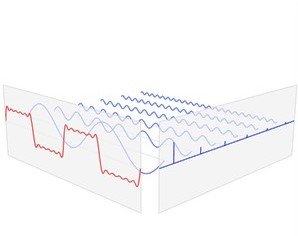
\includegraphics[width=0.45\textwidth]{Images/FT.jpg}
    \caption{Fourier transform.}
    \label{FT}
\end{figure}

In image processing, the discrete Fourier transform (DFT) is often preferred, which takes a finite sequence of equally-spaced values as input and is thus better suited than the FT. It is defined by
\begin{equation}
    X_k = \sum_{n=0}^{N-1} x_n \cdot e^{-i2\pi kn/N}, \quad 0 \leq k \leq N-1,
    \label{FT DFT}
\end{equation}
where $x_0,x_1,...,x_{N-1}$ is the input sequence and $X_0,X_1,...,X_{N-1}$ is the output sequence. $X_k$ is effectively the result of the dot product between the vector $[x_0,x_1,...,x_{N-1}]$ and $[e^0,e^{-i2\pi k/N},...,,e^{-i2\pi k(N-1)/N}]$, and the latter is a finite sequence of frequency $2\pi k$. Therefore, the DFT computes the magnitude of the component of the input sequence with frequency $2\pi k$, for $0 \leq k \leq N-1$.

Fig. \ref{FT FFT on images} gives an example of FFT applied to a real image. The top row shows a set of images and the bottom row shows the corresponding transforms (amplitudes only). Points near the origin represent lower-frequency components and are cut off when a high-pass filter is applied to the image.

\begin{figure}[htbp]
    \centering
    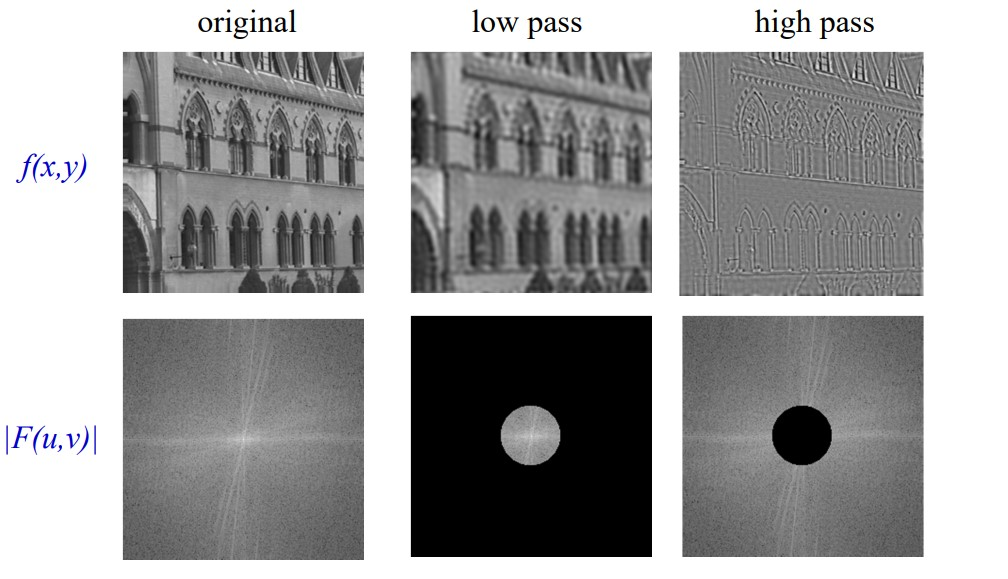
\includegraphics[width=0.45\textwidth]{Images/FFT on images.jpg}
    \caption{FFT and filtering on images \cite{FT lecture}.}
    \label{FT FFT on images}
\end{figure}

A drawback of using \eqref{FT DFT} is that it has a time complexity of $O(N^2)$. In image processing, where the inputs are 2D sequences, the time complexity quickly explodes and makes the equation practically impossible to use. A fast Fourier transform (FFT) is an algorithm that computes the DFT with smaller timer complexity. There are many feasible algorithms and all known ones have complexity $O(N\log N)$. Detailed discussion on FFT algorithms is beyond the scope of this report.

The focusing and astigmatism of an SEM image can be evaluated using its FFT. Fig. \ref{SEM astigmatism} provides a set of sample images that illustrate how different degrees of defocus and astigmatism affect the image and its FFT. An in-focus image contains more details, and its FFT will thus have stronger high-frequency components. As an astigmatic image goes from under-focus from over-focus, the elliptical incidence area of the electron probe rotates by 90 degrees and makes the image appear stretched in the new direction. As a result, its FFT also rotates by 90 degrees.

An image is effectively a finite sequence of data, and this can cause boundary effect when its FFT is calculated. The abrupt discontinuity at the edges gives the FFT some strong high-frequency components. To circumvent this, the \textit{SemImage} class provides two methods --- \lstinline{applyHamming()} and \lstinline{applyHanning()}, which apply a Hamming and Hanning window function to the image data, respectively. The window functions taper the edges off towards zero, and thus reduce the boundary effect. Fig. \ref{Window functions} illustrates how they look like, and they can be obtained by setting $a_0$ to $0.5$ and $25/46$, respectively, in the function
\begin{equation}
    w[n] = a_0 - (1-a_0)\cdot \cos{\frac{2\pi n}{N}}, \quad 0\leq n \leq N.
\end{equation}

\begin{figure}[htbp]
    \centering
    \begin{subfigure}{0.45\textwidth}
        \centering
        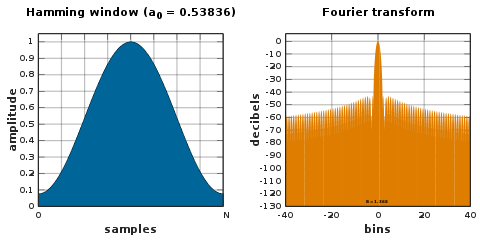
\includegraphics[width=1\textwidth]{Images/Window Hamming.png}
        \caption{Hamming window.}
        \label{Window Hamming}
    \end{subfigure}
    \begin{subfigure}{0.45\textwidth}
        \centering
        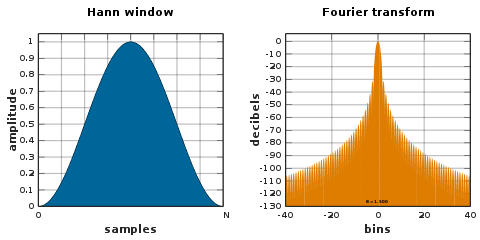
\includegraphics[width=1\textwidth]{Images/Window Hanning.png}
        \caption{Hanning window.}
        \label{Window Hanning}
    \end{subfigure}
    \caption{Window functions.}
    \label{Window functions}
\end{figure}

As summarised in table \ref{Software speed comparison}, the use of GPU can make calculating FFT eight times faster. Without the GPU, calculating FFT alone limits the refresh rate of the tool to 16 frames per second. The GPU improves the number to 125 frames per second.

\begin{figure*}
    \centering
    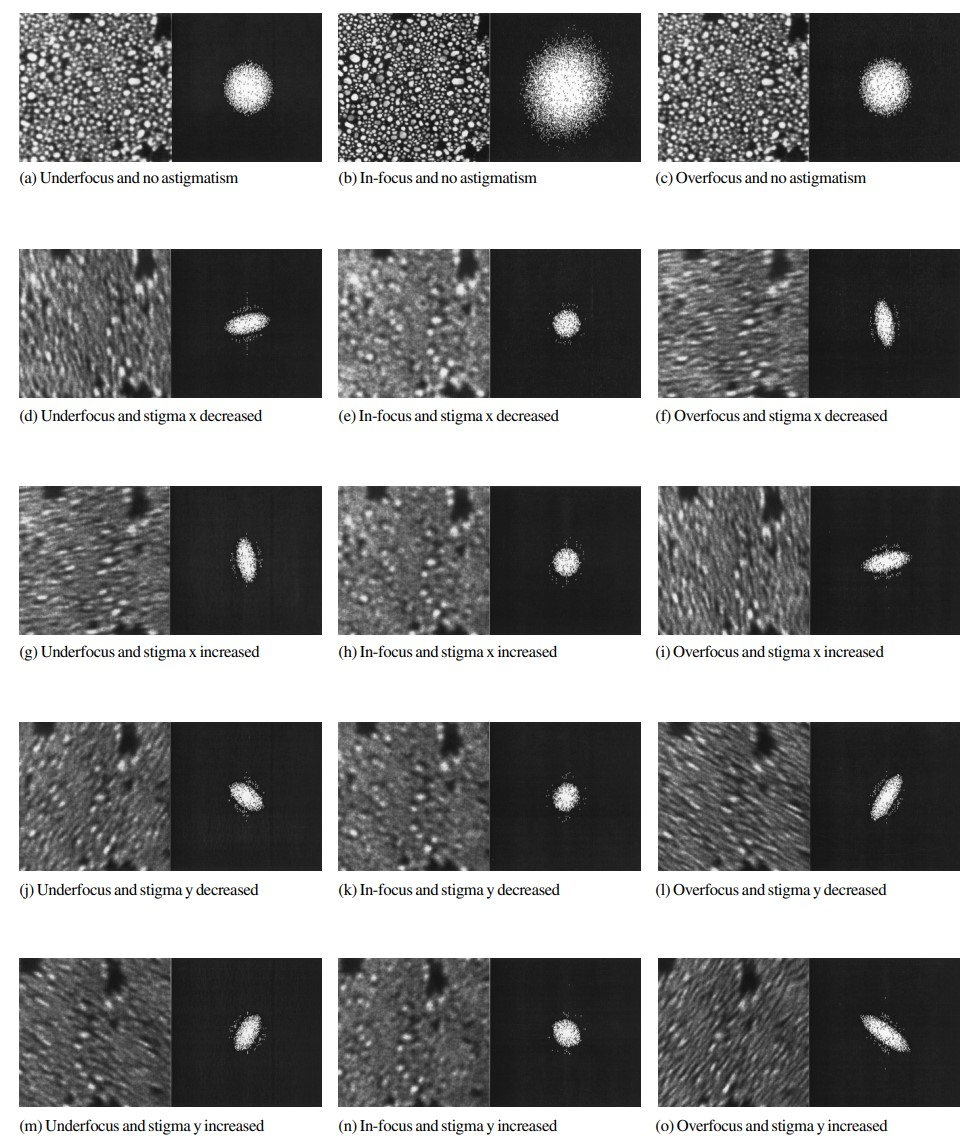
\includegraphics[width=1\textwidth]{Images/SEM astigmatism.jpg}
    \caption{Images of gold-on-carbon sample and their fast Fourier transforms (FFTs) for different degrees of defocus and astigmatism \cite{SEM correction algorithm}.}
    \label{SEM astigmatism}
\end{figure*}

\section{Automatic focusing and astigmatism correction algorithm}
\label{Section correction algorithm}
K.H. Ong, J.C.H. Phang, and J.T.L. Thong proposed an algorithm for automatic focusing and astigmatism correction \cite{SEM correction algorithm} using the properties of the FFT of SEM images described in section \ref{Section FFT}.

The FFT of an image can be converted into a binary image by applying a threshold to the magnitudes, and then segmented into 8 regions as shown in Fig. \ref{FFT regions}. A pixel has value 1 if the magnitude is above the threshold and 0 otherwise. Let $I$ be a matrix representing the current image with focus set to $F$, obtain an under-focused image $I_{uf}$ and an over-focused image $I_{of}$ by setting the focus to $F-\Delta F=F_{uf}$ and $F+\Delta F=F_{of}$, respectively. Let $T$, $T_{uf}$ and $T_{of}$ be matrices representing the binary FFT of $I$, $I_{uf}$ and $I_{of}$, respectively.

\begin{figure}[htbp]
    \centering
    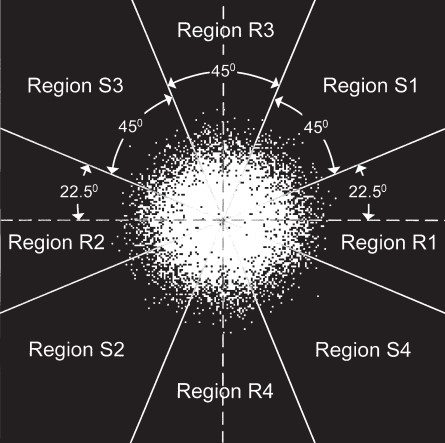
\includegraphics[width=0.4\textwidth]{Images/FFT regions.jpg}
    \caption{Segmented fast Fourier transform \cite{SEM correction algorithm}.}
    \label{FFT regions}
\end{figure}

The focus can be adjusted by comparing the sum of pixel values in $T$, $T_{uf}$ and $T_{of}$. Let the perfect focus for the image be $\hat{F}$, then
\begin{align*}
    \small
\begin{cases}
    \text{sum}(T_{of}) < \text{sum}(T) < \text{sum}(T_{uf}), & \hat{F} < F_{uf} \\
    \text{sum}(T_{of}) < \text{sum}(T_{uf}), & F_{uf} < \hat{F} < F \\
    \text{sum}(T_{of}) = \text{sum}(T_{uf}) < \text{sum}(T), & F = \hat{F} \\
    \text{sum}(T_{uf}) < \text{sum}(T_{of}), & F_{of} > \hat{F} > F \\
    \text{sum}(T_{uf}) < \text{sum}(T) < \text{sum}(T_{of}), & \hat{F} > F_{of}
\end{cases}.
\end{align*}
Let
\begin{equation}
    P = \text{sum}(T_{of}) - \text{sum}(T_{uf}).
\end{equation}
Then, the rules for adjusting focus are
\begin{itemize}
    \item when $P>0$, the focus should be decreased.
    \item when $P<0$, the focus should be increased.
\end{itemize}

After the focus has been set to the perfect value, i.e. when $F=\hat{F}$, the stigmator settings can be determined by comparing the sum of pixel values in different regions of $T$, $T_{uf}$ and $T_{of}$. Let
\begin{align}
    P_{R12} & = \text{sum}(T_{of,R12}) - \text{sum}(T_{uf,R12}), \\
    P_{R34} & = \text{sum}(T_{of,R34}) - \text{sum}(T_{uf,R34}), \\
    P_{S12} & = \text{sum}(T_{of,S12}) - \text{sum}(T_{uf,S12}), \\
    P_{S34} & = \text{sum}(T_{of,S34}) - \text{sum}(T_{uf,S34}).
\end{align}
The rules for adjusting the stigmators can be determined from Fig. \ref{SEM astigmatism}. As can be seen in the figure, stigmator x affects the astigmatism in the horizontal and vertical directions, i.e. $P_{R12}$ and $P_{R34}$, and stigmator y affects that in the diagonal directions, i.e. $P_{S12}$ and ${P_{S34}}$. Then:
\begin{itemize}
    \item when $P_{R12}>0$ and $P_{R34}<0$, the value of stigmator x should be decreased.
    \item when $P_{R12}<0$ and $P_{R34}>0$, the value of stigmator x should be increased.
    \item when $P_{S12}>0$ and $P_{S34}<0$, the value of stigmator y should be increased.
    \item when $P_{S12}<0$ and $P_{S34}>0$, the value of stigmator y should be decreased.
\end{itemize}

Fig. \ref{Correction algorithm flowchart} shows the general flow chart of the algorithm.

\begin{figure}[htbp]
    \centering
    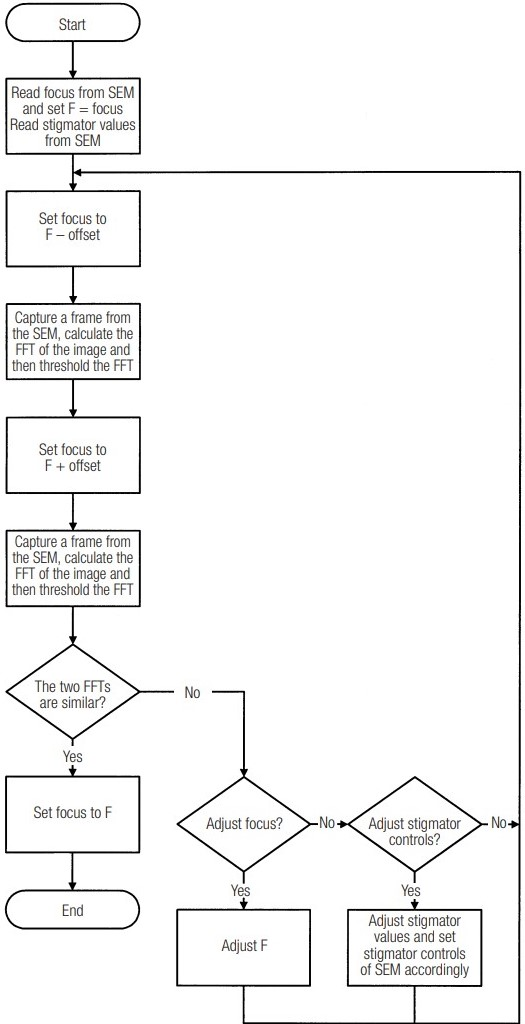
\includegraphics[width=0.48\textwidth]{Images/Correction algorithm flowchart.jpg}
    \caption{General flow chart of the correction algorithm \cite{SEM correction algorithm}.}
    \label{Correction algorithm flowchart}
\end{figure}

The performance of the algorithm is affected by five key parameters:
\begin{itemize}
    \item $P_{threshold}$. Ideally, the focus of the SEM should be set to a value such that $P = 0$, i.e. the under-focused image and the over-focused image have the same FFT magnitude. However, this is practically impossible due to noise, non-linearity in the lens system, etc. Therefore, $P_{threshold}$ is used to define a threshold such that the image is considered to be in perfect focus when $|P| < P_{threshold}$. If $P$ is normalised, $P_{threshold}$ can be conveniently set to a percentage value.
    \item $F_{step}$, which is how much the focus should be adjusted during each iteration in focus adjustment. A smaller $F_{step}$ allows the final image to have a finer resolution but increases the amount of time needed for the adjustment. A larger $F_{step}$ speeds up the process but may never achieve the level of focus as required by $P_{threshold}$. To achieve the best result, larger values of $F_{step}$ should be used at the beginning and smaller ones towards the end.
    \item $\Delta F$, which determines how much the focus should be changed to obtain the under-focused and over-focused images. It is more important to the astigmatism correction step. When $\Delta F$ is too small, the difference between the FFT of the under-focused and over-focused image will not be significant enough and can be easily hidden by noise. When it is too big, the FFTs will lose their high-frequency components, which again makes the difference too small.
    \item $S_{threshold}$. The values of $P_{R12}, P_{R34}, P_{S12}, P_{S34}$ are prone to the influence of noise near zero. Same as the purpose of $P_{threshold}$, $S_{threshold}$ defines a threshold to circumvent this problem.
    \item $S_{step}$, which is how much the value of the stigmator control should be adjusted during each iteration in astigmatism adjustment. Similar to $F_{step}$, it determines the speed of the adjustment and the level of fineness of the final images.
\end{itemize}

Another factor that affects the speed of the automatic focusing and astigmatism correction algorithm is the speed of performing segmentation on the FFTs. The most straightforward way of doing it is to iterate through the whole matrix while calculating the sums in pure Python, for every FFT. This has a time complexity of $O(N^2)$. The \textit{Masker} module provides a faster solution.

A \textit{Masker} can be initialised with a 2D shape, and it will create eight matrices, each representing a region as shown in Fig. \ref{FFT regions}. For example, if the input is $[5, 7]$, the matrix created for region R1 will be
\begin{align*}
\begin{bmatrix}
1 & 1 & 1 & 1 & 1 & 1 & 1\\
1 & 1 & 1 & 1 & 1 & 1 & 0\\
1 & 1 & 1 & 0 & 0 & 0 & 0\\
1 & 1 & 1 & 1 & 1 & 1 & 0\\
1 & 1 & 1 & 1 & 1 & 1 & 1
\end{bmatrix}.
\end{align*}
The code ensures that there is no overlapping between matrices apart from at the center. After obtaining the matrix for region R1, the sum of of values in an FFT in R1 can be calculated using:
\begin{lstlisting}
ma.array(fft, masker.r1).sum()
\end{lstlisting}

The correction algorithm is implemented by the \textit{SemCorrector} class. Due to the impact of the COVID-19 pandemic, only the focusing correction part has been tested and the result is as shown in Fig. \ref{Correction focusing demo}. The algorithm was able to find the same best focus for the SEM as determined by the operator.

\begin{figure}[htbp]
    \centering
    \begin{subfigure}{0.45\textwidth}
        \centering
        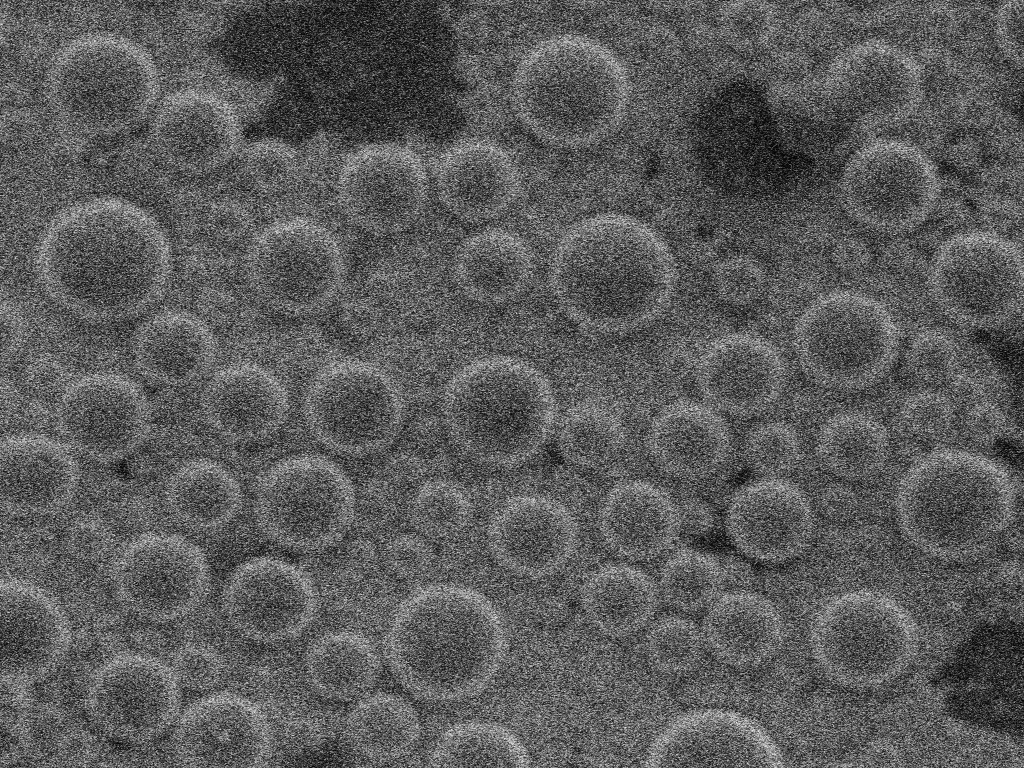
\includegraphics[width=1\textwidth]{Images/Correction initial.png}
        \caption{Initial.}
    \end{subfigure}
    \begin{subfigure}{0.45\textwidth}
        \centering
        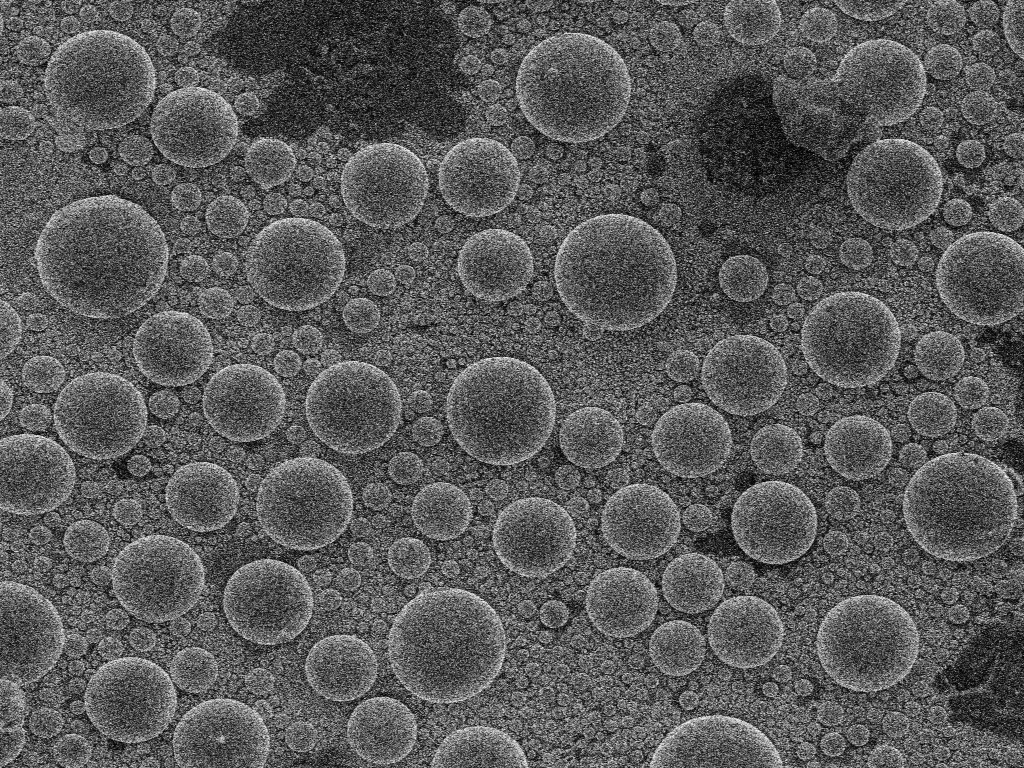
\includegraphics[width=1\textwidth]{Images/Correction final.png}
        \caption{Final.}
    \end{subfigure}
    \caption{Automatic focusing correction.}
    \label{Correction focusing demo}
\end{figure}

The algorithm has two major practical problems. The first one is that it takes time for the SEM image to be updated after a change in the settings has been made. This is because the SEM needs to perform multiple scans on the object and take the average to reduce noise. To obtain an 8-bit 1024 $\times$ 768 image with good quality, the algorithm typically has to wait for a quarter of a second for each iteration. This significantly slows down the speed of the algorithm. A possible solution is to reduce the sample size on the SEM and thereby reducing the time needed for performing the scans.

Another problem is that it is difficult to determine the best values for the five parameters mentioned earlier. The result showed in Fig. \ref{Correction focusing demo} was obtained using the best settings found empirically, which may be dependent on the model of the SEM and characteristics of the object under observation.

\section{Conclusions}
Two image analysis algorithms --- the FFT and histogram equalisation can be performed about eight times faster on the GPU than on the CPU. This has allowed the real-time image diagnostic tool to have a refresh rate of more than ten frames per second, even if it is written in a relatively slow interpreted programming language.

\begin{thebibliography}{00}
    \bibitem{SEM for semiconductors}
    T. Agemura and T. Sekiguchi, "Secondary electron spectroscopy for imaging semiconductor materials," 2018 International Symposium on Semiconductor Manufacturing (ISSM), Tokyo, Japan, 2018, pp. 1-3, doi: 10.1109/ISSM.2018.8651171.

    \bibitem{SEM for bacterial cells}
    T. Cushnie, N. O’Driscoll and A. Lamb, "Morphological and ultrastructural changes in bacterial cells as an indicator of antibacterial mechanism of action," Cellular and Molecular Life Sciences, 2016, vol. 73, no. 23, pp. 4471-4492, doi: 10.1007/s00018-016-2302-2.

    \bibitem{SEM A to Z}
    "SEM A to Z," Jeol.co.jp, [Online], available: \url{https://www.jeol.co.jp/en/applications/pdf/sm/sem_atoz_all.pdf}. [Accessed: 18 May 2020].

    \bibitem{SEM for microstructural analysis}
    E. Ghassemieh, M. Acar and H. Versteeg, "Microstructural analysis of non-woven fabrics using scanning electron microscopy and image processing. Part 1: Development and verification of the methods," Proceedings of the Institution of Mechanical Engineers, Part L: Journal of Materials: Design and Applications, 2002, vol. 216, no. 3, pp. 199-207, doi: 10.1177/146442070221600305.

    \bibitem{SEM image sharpness measurement}
    A. Vladár, M. Postek and M. Davidson, "Image sharpness measurement in scanning electron microscopy-part II," Scanning, 2006, vol. 20, no. 1, pp. 24-34, doi: 10.1002/sca.1998.4950200104.

    \bibitem{GPU mediated reality}
    J. Fung, F. Tang and S. Mann, "Mediated reality using computer graphics hardware for computer vision," Proceedings. Sixth International Symposium on Wearable Computers, Seattle, WA, USA, 2002, pp. 83-89, doi: 10.1109/ISWC.2002.1167222.

    \bibitem{SEM astigmatism correction}
    C. Lyman, "Correcting Astigmatism in SEM Images," Microscopy Today, 2019, vol. 27, no. 03, pp. 32-35, doi: 10.1017/s1551929519000476.

    % \bibitem{Histogram equalisation wiki}
    % "Histogram equalization." en.wikipedia.org. \url{https://en.wikipedia.org/wiki/Histogram_equalization} (accessed May 11, 2020).

    % \bibitem{Fourier transform wiki}
    % "Fourier transform." en.wikipedia.org. \url{https://en.wikipedia.org/wiki/Fourier_transform} (accessed May 12, 2020).

    \bibitem{FT lecture}
    "2D Fourier transforms and applications," University of Oxford, 2014, [Online], available: \url{http://www.robots.ox.ac.uk/}. [Accessed: 19 May 2020].

    % \bibitem{Fast Fourier transform wiki}
    % "Fast Fourier transform." en.wikipedia.org. \url{https://en.wikipedia.org/wiki/Fast_Fourier_transform} (accessed May 12, 2020).
    
    \bibitem{SEM correction algorithm}
    K.H. Ong, J.C.H. Phang and J.T.L. Thong, "A robust focusing and astigmatism correction method for the scanning electron microscope," 1997, scanning 19: 553-563, doi: 10.1002/sca.4950190805.

    % \bibitem{Window function wiki}
    % "Window function." en.wikipedia.org. \url{https://en.wikipedia.org/wiki/Window_function} (accessed May 13, 2020).
\end{thebibliography}
\end{document}
